\documentclass[twoside,twocolumn]{article}

\usepackage{blindtext} 
\usepackage{graphicx}
\usepackage[sc]{mathpazo} 
\usepackage[T1]{fontenc} 
\linespread{1.05} 
\usepackage{microtype} 

\usepackage[english]{babel} 

\usepackage[hmarginratio=1:1,top=32mm,columnsep=20pt]{geometry} 
\usepackage[hang, small,labelfont=bf,up,textfont=it,up]{caption} 
\usepackage{booktabs} 

\usepackage{lettrine} 

\usepackage{enumitem} 
\setlist[itemize]{noitemsep} 

\usepackage{abstract} 
\renewcommand{\abstractnamefont}{\normalfont\bfseries} 
\renewcommand{\abstracttextfont}{\normalfont\small\itshape} 

\usepackage{titlesec} 
\renewcommand\thesection{\Roman{section}} % 
\renewcommand\thesubsection{\roman{subsection}} 
\titleformat{\section}[block]{\large\scshape\centering}{\thesection.}{1em}{} 
\titleformat{\subsection}[block]{\large}{\thesubsection.}{1em}{} 

\usepackage{fancyhdr} 
\pagestyle{fancy} 
\fancyhead{} 
\fancyfoot{} 
\fancyhead[C]{Titulo $\bullet$ Junio 2019 $\bullet$ } 
\fancyfoot[RO,LE]{\thepage} 

\usepackage{titling} 

\usepackage{hyperref} 

%----------------------------------------------------------------------------------------
%	TILULOS
%----------------------------------------------------------------------------------------

\setlength{\droptitle}{-4\baselineskip} 

\pretitle{\begin{center}\Huge\bfseries} 
\posttitle{\end{center}} 
\title{Titulo del articulo} 
\author{Andre Reinoso Aranda, Marko Antonio Rivas Rios, Andree Velasco Sucapuca, \\
Percy Taquila Carazas }
\date{\today} 
\renewcommand{\maketitlehookd}{
\begin{abstract}
\noindent 
Abstract en ingles
\end{abstract}
\begin{abstract}
\noindent 
Abstract en español
\end{abstract}
}

%----------------------------------------------------------------------------------------

\begin{document}

% Print the title
\maketitle

%----------------------------------------------------------------------------------------
%	INTRODUCCION
%----------------------------------------------------------------------------------------

\section{Introduccion}
\lettrine[nindent=0em,lines=3]{A}ctualmente en el Perú las pequeñas y medianas empresas producen al mercado peruano ingresos y empleo, la gran cantidad de informacion que manejan es debido al alto numero de operaciones que realizan a diario.\\ \\
El aumento de competencia hace que el area administrativa tome decisiones a base de su experiencia, publicidad, tecnologia, recursos humanos y hasta de su propia intuicion.\\ \\
Sin embargo hay empresas que no toman de manera estructurada las decisiones, o no implementan herramientas de Business Intelligence que permitirian al gerente escenarios, reportes, etc. una mejor toma de deciciones respecto a su rubro. \\ \\
Aquella empresa que si lleva a cabo procesos de extraccion de datos, transformacion de datos, uso de herramientas y metodos, tendra una ventaja notoria a comparacion de las demas que no lo aplican.
\\ \\
El Business Analytics busca trabajar los datos con conceptos estadisticos, modelos analiticos, permitiendo la elaboracion de escenarios con las que las organizacion tomen decisiones anticipandoce a lo que vendra a futuro. El Business Analytics busca la simulacion de procesos, el desarrollo de escenarios, predicciones, relaciones entre las areas de una organizacion, etc.

%----------------------------------------------------------------------------------------
%	Objetivos
%----------------------------------------------------------------------------------------

\section{Marco teorico}

\begin{itemize}
\item Aqui
\item Aqui

\end{itemize}



%----------------------------------------------------------------------------------------
%	DESARROLLO
%----------------------------------------------------------------------------------------

\section{Desarrollo}

\subsection{¿Que es la inteligencia de negocios?}

La informacion ha propiciado la necesidad de tener mejores, mas rapidos y mas eficientes metodos para extraer y transformar los datos de una organizacion en informacion.
\\ \\
En 1958 \textbf{Hans Peter Luhn}, investigador de la IBM, acuña el termino en el articulo "A Business Intelligence System":
\\ \\
\textsl{''La habilidad de aprender las relaciones de hechos presentados de forma que guien las acciones hacia una meta deseada''}
\\ \\
En 1989 \textbf{Howard Dresden}, analista de Gartner, propone una definicion formal del concepto.
\\ \\
\textsl{"Conceptos y métodos para mejorar la toma de decisiones comerciales mediante el uso de un sistema de soporte basado en hechos''}
\\ \\
En pocas palabras: \\ \\
\textbf{Es el conjunto de metedologias, aplicaciones, capacidades administrativas de informacion que permite tomar mejores decisiones a los usuarios de una organizacion.}


\subsection{¿Cuando aplicar la inteligencia de negocios?}

Contenido

\subsection{¿Qué ventajas nos da usar la inteligencia de negocios?}

- Nos permite tomar decisiones rápidas. \\
- Ayuda a definir escenarios adecuados. \\
- Permite tomar la información, la convierte en conocimiento para la toma de decisiones. \\
\subsection{Beneficions de la inteligencia de negocios}

- Beneficios tangibles, por ejemplo: reducción de costes, generación de ingresos, reducción de tiempos para las distintas actividades del negocio. \\\\
- Beneficios intangibles: el hecho de que tengamos disponible la información para la toma de decisiones hará que más usuarios utilicen dicha información para tomar decisiones y mejorar la nuestra posición competitiva, por ejemplo: Cuales son los horarios en que más visitan la tienda, cual es el recorrido que hacen en el interior del local. \\\\
- Beneficios estratégicos: Todos aquellos que nos facilitan la formulación de la estrategia, es decir, a qué clientes, mercados o con qué productos dirigirnos, por ejemplo: ofertas que más solicitan los clientes. \\\\

\subsection{¿Que es el análisis de negocio?}

Es la exploración iterativa y metódica de los datos de una organización, resaltando el análisis estadístico. El análisis empresarial es usado por empresas que toman decisiones basadas en datos. 
\\ \\
Las empresas basadas en datos tratan sus datos como un activo corporativo y buscan convertirlos en una ventaja competitiva. El análisis empresarial depende de la calidad de los datos, de los analistas expertos que entienden las tecnologías y el negocio, y el compromiso de la organización de utilizar los datos para obtener información que ayude en las decisiones comerciales.
\\ \\
Bussiness analytics, se define como el campo del análisis empresarial, se trata del proceso de recopilación, almacenamiento y análisis de datos para asesorar a una empresa mejorando su eficiencia para aumentar sus ingresos.
\\ \\
Si una empresa usa un enfoque que se base en datos en su proceso de toma de decisiones, da como resultado que el análisis juega un rol de gran importancia para la toma de decisiones.  Las personas especialistas en este tema se llaman \textbf{ “Analistas Empresariales”}
\\ \\
Las instituciones recopilan y almacenas datos durante muchos años, pero en los últimos años, han aumentado en cantidad significativa pero la mayor parte de estos datos no están estructurados.  
\\ \\
Según \textbf{MarTech}
\textsl{“El universo digital tiene 2,7 Zettabytes de datos, y si la mayor parte no está estructurada, analizarlo requerirá muchos analistas de datos.  No es de extrañar que el gasto en proyectos de bigdata (proyectos de análisis de negocios) en el 2018 alcanzó los \$114 mil millones de dólares."}

\subsection{Función del análisis de negocio}
Cuando se determina el objetivo comercial del análisis, se selecciona una metodología de análisis y se adquieren datos para respaldar dicho análisis.  Esta adquisición de datos implica la extracción de uno o más sistemas comerciales, la limpieza y la integración en un único almacén de datos.
\\ \\
Este análisis inicial se realiza con una muestra pequeña de datos.  Las herramientas que se utilizan van desde hojas de cálculo, estadística, aplicaciones complejas de extracción de datos y modelado predictivo. A medida que se van descubriendo patrones y relaciones, se hacen nuevas preguntas, completando el proceso analítico, hasta que se cumpla el objetivo comercial.
\\ \\
El despliegue de modelos predictivos implican la puntuación de registros de datos, generalmente en una base de datos, el uso de los puntajes son para optimizar las decisiones en tiempo real, dentro de las aplicaciones y los procesos comerciales del BA, además ayuda en la toma de decisiones tácticas en respuesta a eventos imprevistos.  Y en muchos casos, hasta la toma de decisiones esta automatizada para admitir respuestas en tiempo real.
\subsection{Tipos de análisis de negociol}
Los tipos específicos de análisis de negocios incluyen:

\begin{itemize}	

	\item \textbf{Análisis descriptivo}: Rastrea los indicadores clave de rendimiento (KPI) para comprender el estado actual de un negocio.
	\item \textbf{Análisis predictivo}: Analiza los datos de tendencias para evaluar la probabilidad de resultados futuros.
	\item \textbf{Análisis prescriptivo}: Utiliza el rendimiento pasado para generar recomendaciones sobre cómo manejar situaciones similares en el futuro.

\end{itemize} 



\subsection{Titulo Nr8}
Contenido 


\subsection{Titulo Nr9}
Contenido 



\subsection{Titulo Nr10}
Contenido 

\begin{center}
	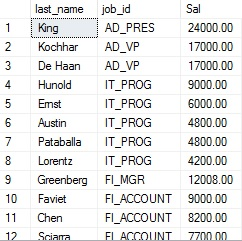
\includegraphics[width=7cm]{./Imagenes/img} 
\end{center}

%----------------------------------------------------------------------------------------
%	CONCLUSIONES
%----------------------------------------------------------------------------------------

\section{Conclusiones}

Aqui van las conclusiones


%----------------------------------------------------------------------------------------
%	BIBLIOGRAFIA
%----------------------------------------------------------------------------------------

\begin{thebibliography}{99} 

\bibitem[Silvia Chavez y Carmen Contreras, 2018]{}
\newblock Implementación de Business Intelligence, para el proceso de toma de decisiones del área de ventas.

\bibitem[Alex Rayón, 2015]{Universidad de Deusto}
Conceptos básicos del Business Intelligence.

\bibitem[Jordi Conesa y Josep Curto, 2010]{}
\newblock Introduccion al Business Intelligence

\bibitem[Margaret Rouse, 2019]{}
\newblock Análisis de negocios (BA)

\bibitem[Noodle Editorial Staff, 2018]{}
\newblock Business analytics career paths

\bibitem[Josep Lluis Cano, 2007]{}
\newblock Business Intelligence: competir con información
 

 
\end{thebibliography}

%----------------------------------------------------------------------------------------

\end{document}
